%-*-coding: utf-8-*-
\FloatBarrier
\chapter{Обзор предметной области}

В данной главе приводятся необходимые определения, постановка задачи, проводится обзор существующих алгоритмов решения поставленной задачи.
% , а также смежных задач в предметной области.

\FloatBarrier
\section{Основные определения}

Введем необходимые формальные определения, которые будут использоваться в дальнейшем.

\subsection{Филогенетика}

\emph{Филогенетика} --- область биологической систематики, которая занимается идентификацией и прояснением эволюционных взаимоотношений среди разных видов жизни на Земле~\cite{wiki:phylogenetics}.

\emph{Филогенетическим деревом} называется дерево, отражающее эволюционные взаимосвязи между различными видами или другими сущностями, имеющими общего предка~\cite{wiki:phylogenetic-tree}.
В данной работе будут рассматриваться подвешенные двоичные деревья. Листья филогенетического дерева отображают таксоны, а узлы представляют из себя эволюционные события: разделение предкового вида на два независимых.
Примеры филогенетических деревьев показаны на Рис.~\ref{input-example}.

\emph{Гибридизационная сеть} --- направленный ациклический граф с выделенным корнем.
Гибридизационная сеть состоит из трех типов вершин - обычных вершин, ретикулярных вершин и листьев.
Обычные вершины имеют одного предка и нескольких потомков.
\emph{Ретикулярные вершины} имеют более одного предка и нескольких потомков.
Листья имеют одного предка и не имеют потомков.
В данной работе, без потери общности, будет рассматриваться упрощенная модель гибридизационной сети, в которой обычные вершины имеют ровно двух потомков, а ретикулярные вершины имеют ровно двух предков и ровно одного потомка. 
Заметим, что привести произвольную гибридизационную сеть к упрощенному виду не составляет труда~\cite{wu2010close}.
Примеры гибридизационных сетей показаны на Рис.~\ref{network-example}.

\begin{figure}[t]
  \centering
  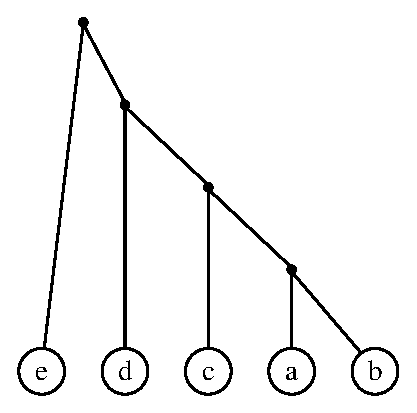
\includegraphics[width=4cm]{img/inp1.eps}
  \hspace{5mm}
  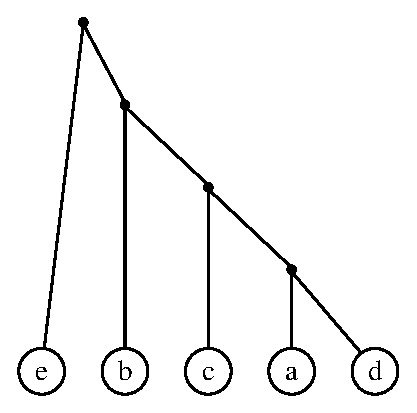
\includegraphics[width=4cm]{img/inp2.eps}
  \hspace{5mm}
  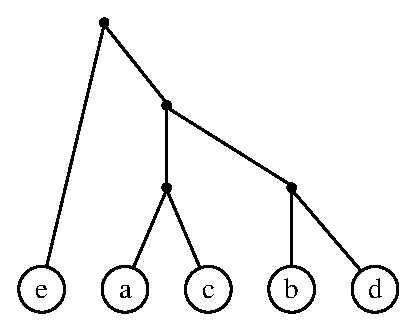
\includegraphics[width=4cm]{img/inp3.eps}
  \caption{Три филогенетических дерева над множеством таксонов \{a, b, c, d, e\}.}
  \label{input-example}
\end{figure}

\begin{figure}[t]
  \centering
  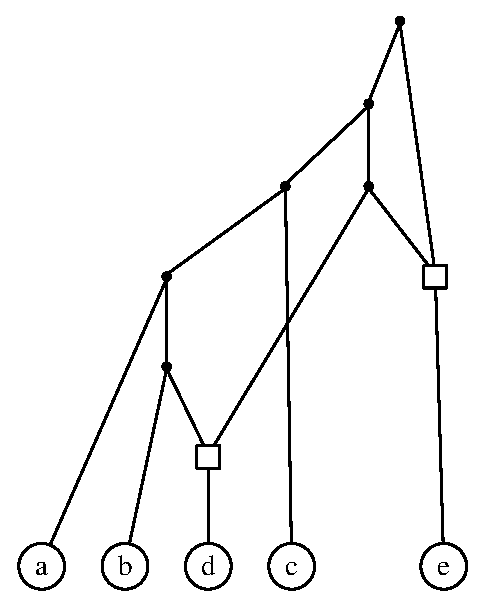
\includegraphics[width=4cm]{img/ans.eps}
  \hspace{1cm}
  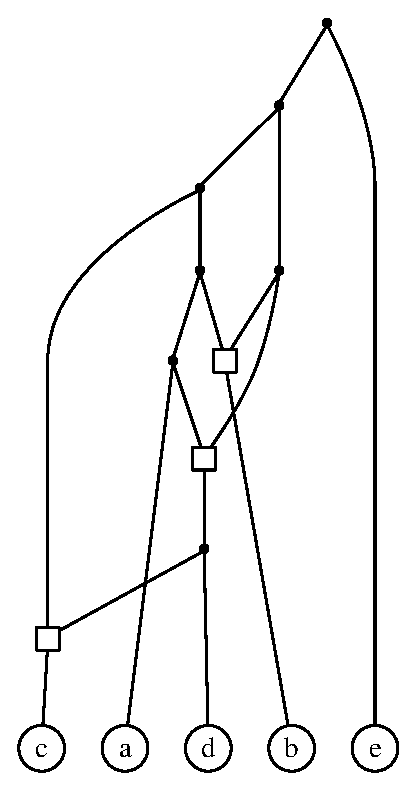
\includegraphics[width=4cm]{img/ans3.eps}
  \caption{Возможные гибридизационные сети, для деревьев из Рис.~\ref{input-example}, с двумя и тремя ретикулярными событиями соответственно. Ретикулярные вершины обозначены квадратиками.}
  \label{network-example}
\end{figure}

Гибридизационную сеть можно свести к филогенетическому дереву следующим образом:

\begin{itemize}
	\item У каждой ретикулярной вершины необходимо выбрать используемого предка, а ребро ведущее к другому предку удалить.
	\item Если у ретикулярной вершины удалено ребро, ведущее в ее единственного сына, то ретикулярную вершину также следует удалить.
	\item Стянуть все ребра, имеющие ровно одного предка и ровно одного потомка.
\end{itemize}

Гибридизационная сеть $N$ \emph{отображает} дерево $T$, если существует такой способ выбора удаляемых ребер, что после стягивания получится дерево $T'$ изоморфное дереву $T$.
При этом, вершины сети, которые остались после стягивания ребер, будем называть вершинами \emph{используемыми для отображения} дерева $t$.
Гибридизационные сети на Рис.~\ref{network-example} содержат в себе все три дерева из Рис.~\ref{input-example}.

\emph{Гибридизационным числом} сети $N$ с корнем $\rho$ называется величина $h(N) = \sum\limits_{v \ne \rho} (d^-(v) - 1)$, где за $d^-(v)$ обозначена входящая степень вершины $v$.
Аналогично обозначим за $d^+(v)$ исходящую степень вершины $v$.
Заметим, что в нашей модели значение $h(N)$ равно количеству ретикулярных вершин.

Рассмотрим множество из $k$ филогенетических деревьев $T_1, T_2, \dots, T_k$, построенных над фиксированным множеством таксонов.
Сеть $N_{min}$ называется \emph{минимальной гибридизационной сетью}, если она принадлежит множеству сетей, содержащих в себе все $k$ деревьев, и при этом имеет наименьшее возможное гибридизационное число.

Множество таксонов $A$ называется \emph{кластером} на деревьях $T_1, T_2, \dots, T_k$, если в каждом дереве $T_i$ существует вершина $v_i$, такая, что множество листьев в поддереве $v_i$ совпадает с множеством $A$.

\subsection{Выполнимость булевой формулы}

\emph{Задача о выполнимости булевой формулы (SAT)} заключается в следующем: можно ли назначить всем переменным, встречающимся в формуле, значения ложь и истина так, чтобы формула стала истинной~\cite{wiki:sat}. Обычно рассматриваются формулы в конъюктивной нормальной форме.

\emph{SAT-солвер} --- программа предназначенная для решения задачи выполнимости булевой формулы.

% \FloatBarrier
% \section{Обзор смежных исследований}

\FloatBarrier
\section{Постановка задачи}

Задача построения минимальной гибридизационной сети заключается в том, чтобы для множества филогенетических деревьев $T_1, T_2, \dots, T_k$ построить минимальную гибридизационную сеть.

Было показано, что даже для случая двух деревьев эта задача NP-полна~\cite{bordewich2007computing}.

\FloatBarrier
\section{Обзор существующих методов}

Часто, для решения задачи используются различные ухищрения, например расматриваются сети с различными структурные допущениями, например <<galled networks>>~\cite{huson2007beyond} или $k$-уровневые сети~\cite{van2009constructing}. Кроме того, часто допускается, что сеть строится только по двум деревьям~\cite{albrecht2012fast, wu2010fast}. Алгоритмы с такими допущениями рассматриваться не будут. Рассмотрим только алгоритмы, решающие поставленную задачу без допущений.

\subsection{PIRN$_\mathrm{C}$}

Единственный алгоритм, позволяющий гарантированно находить минимальную гибридизационную сеть для произвольного количества входных деревьев.
Будет использоваться для сравнения с точной версией представленного алгоритма.

\subsection{PIRN$_\mathrm{CH}$}

Эвристическая версия алгоритма PIRN$_\mathrm{C}$.
Не гарантирует нахождение точного решения.
Будет использоваться для сравнения с неточной версией представленного алгоритма.

\subsection{MURPAR}

Быстрый эвристический алгоритм основанный на сведении к задаче линейного программирования.
Не гарантирует нахождения точной минимальной сети, но позиционируется как очень быстрый алгоритм для нахождения точной верхней границы гибридизационного числа.
